\documentclass[../main.tex]{subfiles}
\graphicspath{{\subfix{../images/}}}
\begin{document}

Nutrition test of the Swiss Society of Nutrition~\cite{SGE}. Analyze your nutritional habits.

\vspace{5mm}

\textbf{By filling out this questionnaire below, you easily find out in which areas your nutritional habits leaves room for improvement
  and therefore a change is especially important.}

\vspace{5mm}

Maybe you think now: ``But I already know that for a long time!''
Let yourself be surprised, maybe is what you perceived as a big weakness in your nutrition as not even that problematic!

On the other side you might have some ``blind spots in your perception'' (like most people),
nutritional habits which are ingrained and ``guilty pleasures'' which you might not even have considered before.
That might mean, that a change doesn't even have to start, where you always thought it would have to.

\newpage

\section{How do my eating habits look like?}

\vspace{5mm}


\begin{longtable}{rp{8cm}|l|l|l|l|p{4mm}|}
  & \textbf{This statement fits} &
      \STAB{\rotatebox[origin=c]{90}{\textbf{totally}}} &
    \STAB{\rotatebox[origin=c]{90}{\textbf{more or less}}} &
    \STAB{\rotatebox[origin=c]{90}{\textbf{mostly not}}} &
    \STAB{\rotatebox[origin=c]{90}{\textbf{not at all}}} & \\
    \toprule
    \endhead
    1 & I take sufficient time for my meals and eat slowly &
    \qedsymbol{} & \qedsymbol{} & \qedsymbol{} & \qedsymbol{} & \\  \cline{7-7}
        2 & I consciously only eat rarely fatty meats and sausages &
    \qedsymbol{} & \qedsymbol{} & \qedsymbol{} & \qedsymbol{} & \\  \cline{7-7}
    3 & I pay attention that my foods are as much as possible from the region and
    are seasonally available &
    \qedsymbol{} & \qedsymbol{} & \qedsymbol{} & \qedsymbol{} & \\  \cline{7-7}
        4 & I can most of the time enjoy my meals &
    \qedsymbol{} & \qedsymbol{} & \qedsymbol{} & \qedsymbol{} & \\  \cline{7-7}
        5 & I have enough movement, even if the weather is bad &
    \qedsymbol{} & \qedsymbol{} & \qedsymbol{} & \qedsymbol{} & \\  \cline{7-7}
        6 & Even in periods of urgent work, I take the time for breaks for meals &
    \qedsymbol{} & \qedsymbol{} & \qedsymbol{} & \qedsymbol{} & \\  \cline{7-7}
        7 & I make a shopping list before going shopping &
    \qedsymbol{} & \qedsymbol{} & \qedsymbol{} & \qedsymbol{} & \\  \cline{7-7} 
 8 & I consume mostly foods from organic agriculture &
    \qedsymbol{} & \qedsymbol{} & \qedsymbol{} & \qedsymbol{} & \\  \cline{7-7}
9 & I know the approximate fat content of the foods I eat &
    \qedsymbol{} & \qedsymbol{} & \qedsymbol{} & \qedsymbol{} & \\  \cline{7-7}
 10 & It happens that I overeat and then have a feeling of postprandial fullness &
 \cellcolor{lightgray} \qedsymbol{} & \cellcolor{lightgray} \qedsymbol{} &
 \cellcolor{lightgray} \qedsymbol{} & \cellcolor{lightgray} \qedsymbol{} & \\  \cline{7-7}
 11 & I often eat out of frustration, while having stress or when I'm lonely &
 \cellcolor{lightgray} \qedsymbol{} & \cellcolor{lightgray} \qedsymbol{} &
 \cellcolor{lightgray} \qedsymbol{} & \cellcolor{lightgray} \qedsymbol{} & \\  \cline{7-7}
12 & I walk places as often as possible &
    \qedsymbol{} & \qedsymbol{} & \qedsymbol{} & \qedsymbol{} & \\  \cline{7-7}
13 & I use little salt, all purpose savory seasoning or broth and instead spices and herbs &
    \qedsymbol{} & \qedsymbol{} & \qedsymbol{} & \qedsymbol{} & \\  \cline{7-7}
14 & I eat 5 servings of fruits and vegetables a day &
    \qedsymbol{} & \qedsymbol{} & \qedsymbol{} & \qedsymbol{} & \\  \cline{7-7}
15 & I often eat my lunch while walking or standing at the food stall &
\cellcolor{lightgray} \qedsymbol{} & \cellcolor{lightgray} \qedsymbol{} &
\cellcolor{lightgray} \qedsymbol{} & \cellcolor{lightgray} \qedsymbol{} & \\  \cline{7-7}
16 & I prefer whole grain products, like whole grain breads and pasta, brown rice or legumes &
    \qedsymbol{} & \qedsymbol{} & \qedsymbol{} & \qedsymbol{} & \\  \cline{7-7}
 17 & I don't take the elevator a lot. Climbing stairs is good for me &
    \qedsymbol{} & \qedsymbol{} & \qedsymbol{} & \qedsymbol{} & \\  \cline{7-7}
 18 & I often self medicate with food or alcohol when angry or sad &
 \cellcolor{lightgray} \qedsymbol{} & \cellcolor{lightgray} \qedsymbol{} &
 \cellcolor{lightgray} \qedsymbol{} & \cellcolor{lightgray} \qedsymbol{} & \\  \cline{7-7}
19 & I eat 3 servings of milk or milk products a day &
    \qedsymbol{} & \qedsymbol{} & \qedsymbol{} & \qedsymbol{} & \\  \cline{7-7}
20 & I have a sweet tooth, I can barely resist temptations like ice cream, pie, cookies or sweets &
\cellcolor{lightgray} \qedsymbol{} & \cellcolor{lightgray} \qedsymbol{} &
\cellcolor{lightgray} \qedsymbol{} & \cellcolor{lightgray} \qedsymbol{} & \\  \cline{7-7}
21 & I eat a snack between my meals every day, even if I'm not hungry &
\cellcolor{lightgray} \qedsymbol{} & \cellcolor{lightgray} \qedsymbol{} &
\cellcolor{lightgray} \qedsymbol{} & \cellcolor{lightgray} \qedsymbol{} & \\  \cline{7-7}
22 & I prefer studying the menu, instead of just choosing the menu of the day or known dishes &
    \qedsymbol{} & \qedsymbol{} & \qedsymbol{} & \qedsymbol{} & \\  \cline{7-7}
23 & I seldom drink more than \SI{1}{\liter} (\SI{4}{\cup}) a day &
\cellcolor{lightgray} \qedsymbol{} & \cellcolor{lightgray} \qedsymbol{} &
\cellcolor{lightgray} \qedsymbol{} & \cellcolor{lightgray} \qedsymbol{} & \\  \cline{7-7}
24 & I eat at least twice a week a meal like french fries, fried fish or chicken &
\cellcolor{lightgray} \qedsymbol{} & \cellcolor{lightgray} \qedsymbol{} &
\cellcolor{lightgray} \qedsymbol{} & \cellcolor{lightgray} \qedsymbol{} & \\  \cline{7-7}
25 & Sometimes I encourage friends to common sport activities &
    \qedsymbol{} & \qedsymbol{} & \qedsymbol{} & \qedsymbol{} & \\  \cline{7-7}
26 & Fish is part of my diet on a weekly base &
    \qedsymbol{} & \qedsymbol{} & \qedsymbol{} & \qedsymbol{} & \\  \cline{7-7}
27 & While shopping, I make note of the energy and nutrient content of the food &
    \qedsymbol{} & \qedsymbol{} & \qedsymbol{} & \qedsymbol{} & \\  \cline{7-7}
28 & I seldom buy ready to eat meals, I prefer raw, untreated ingredients &
    \qedsymbol{} & \qedsymbol{} & \qedsymbol{} & \qedsymbol{} & \\  \cline{7-7}
 29 & A relax mood while eating is important for me &
    \qedsymbol{} & \qedsymbol{} & \qedsymbol{} & \qedsymbol{} & \\  \cline{7-7}
 30 & I do actively sports and 1--2 a week  or I have in my daily life ongoing phases of movement &
    \qedsymbol{} & \qedsymbol{} & \qedsymbol{} & \qedsymbol{} & \\  \cline{7-7}
    31 & I avoid foods with high sugar content (lemonades, nectar juices, sweets, sweetened cereals,\ldots) &
    \qedsymbol{} & \qedsymbol{} & \qedsymbol{} & \qedsymbol{} & \\  \cline{7-7}
    32 & A piece of meat a day is a must for me &
\cellcolor{lightgray} \qedsymbol{} & \cellcolor{lightgray} \qedsymbol{} &
\cellcolor{lightgray} \qedsymbol{} & \cellcolor{lightgray} \qedsymbol{} & \\  \cline{7-7}
        33 & If I'm not hungry, I normally don't eat anything &
    \qedsymbol{} & \qedsymbol{} & \qedsymbol{} & \qedsymbol{} & \\  \cline{7-7}
    34 & Eating is important in my life &
    \qedsymbol{} & \qedsymbol{} & \qedsymbol{} & \qedsymbol{} & \\  \cline{7-7}
        35 & I need physical activity, laziness is a taboo for me &
    \qedsymbol{} & \qedsymbol{} & \qedsymbol{} & \qedsymbol{} & \\  \cline{7-7}
        36 & I prefer a mode of preparation, which is low on fats used (steam, cook) &
    \qedsymbol{} & \qedsymbol{} & \qedsymbol{} & \qedsymbol{} & \\  \cline{7-7}
    \bottomrule
    \multicolumn{2}{l}{\textbf{Total points}} \\
\end{longtable}

\section{Scoring}

For the questions on white background, ``totally'' gives 4 points, ``more or less'' 3, ``mostly not'' 2 and ``not at all'' 1 point.
For the questions in gray, it's the opposite:  ``totally'' is 1 point, ``more or less'' 2, ``mostly not'' 3 and ``not at all'' 4 points.

\vspace{2mm}

\subsection{Evaluation per Domain}

\begin{tabular}{l|p{10mm}|p{10mm}|p{10mm}|p{10mm}|p{10mm}|p{10mm}||l|}
  & & & & & & & \textbf{Total} \\ \hline
  \cellcolor{lightgray} Question & \cellcolor{lightgray} 14 &
  \cellcolor{lightgray} 19 & \cellcolor{lightgray} 23 &
  \cellcolor{lightgray} 26 & \cellcolor{lightgray} 32 &
& \\
  \textbf{Food pyramid} & & & & & & & \\ [2ex] \hline
  \cellcolor{lightgray} Question & \cellcolor{lightgray} 2
  & \cellcolor{lightgray} 9 & \cellcolor{lightgray} 16 &
  \cellcolor{lightgray} 20 & \cellcolor{lightgray} 24 &
  \cellcolor{lightgray} 31 & \\
  \textbf{Nutrient content} & & & & & & & \\[2ex] \hline
  \cellcolor{lightgray} Question & \cellcolor{lightgray} 7 &
  \cellcolor{lightgray} 13 & \cellcolor{lightgray} 27 &
  \cellcolor{lightgray} 36 & & & \\
  \textbf{Menu planning} & & & & & & & \\[2ex] \cline{1-5} \cline{8-8}
  \cellcolor{lightgray} Question & \cellcolor{lightgray} 1 & \cellcolor{lightgray} 10
  & \cellcolor{lightgray} 21 & \cellcolor{lightgray} 33 & 
  &   & \\
  \textbf{Nutritional habits} & & & & & & & \\[2ex] \cline{1-5} \cline{8-8}
  \cellcolor{lightgray} Question & \cellcolor{lightgray} 3 & \cellcolor{lightgray} 8 &
  \cellcolor{lightgray} 28 & & & & \\

  \textbf{Season and Environment} & & & & & & & \\[2ex] \cline{1-5} \cline{8-8}
  \cellcolor{lightgray} Question & \cellcolor{lightgray} 4 & \cellcolor{lightgray} 15 &
  \cellcolor{lightgray} 22 & \cellcolor{lightgray} 34 & & & \\
  \textbf{Enjoyment} & & & & & & & \\ [2ex] \hline
  \cellcolor{lightgray} Question & \cellcolor{lightgray} 5 & \cellcolor{lightgray} 12 &
  \cellcolor{lightgray} 17 & \cellcolor{lightgray} 25 & \cellcolor{lightgray} 30 &
  \cellcolor{lightgray} 35 & \\
  \textbf{Exercise} & & & & & & & \\ [2ex]\hline
  \cellcolor{lightgray} Question & \cellcolor{lightgray} 6 & \cellcolor{lightgray} 11 &
  \cellcolor{lightgray} 18 & \cellcolor{lightgray} 29 & &
 & \\
  \textbf{Relaxation} & & & & & & & \\ [2ex] \cline{1-5} \cline{8-8}

\end{tabular}

\subsection{Room for Improvement at a Glance}

Color or cross off the numbers up to the achieved score in each domain.

%Write the points scored for each question in the space provided after the question and tally your point score up. Note your total score under total points at the end of the questionnaire.

\noindent 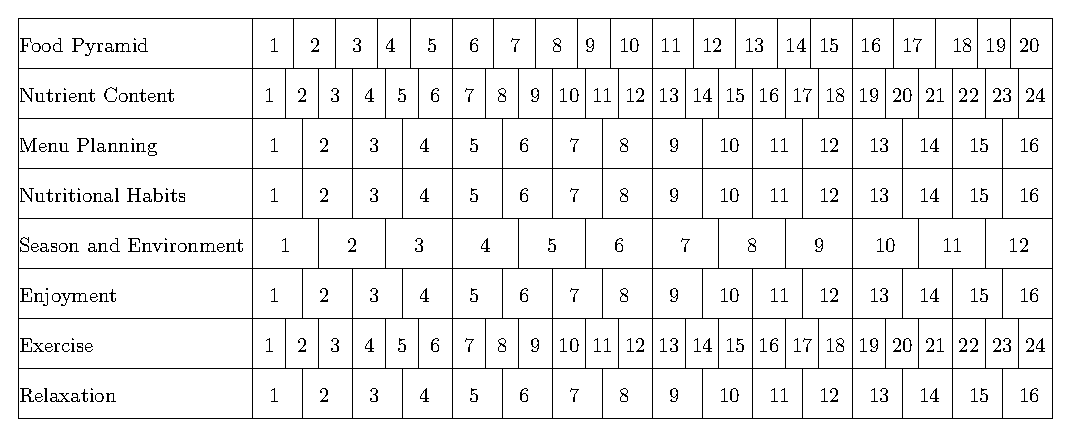
\includegraphics[width=\linewidth]{ImprovementNutr}

\section{The Different Types of Eating Habits}

\noindent \textbf{36--62 Points = ``Impulsive Eater''}

\noindent  \emph{(Considering healthy nutrition and tailored to suit to your needs is not important for you)}

\vspace{2mm}

  You don't care much, if what you eat is conductive for your health.
  You have your  own style of eating and so far didn't put any thought on adapting it to a healthy and weight conscious nutrition.
  When you start making small but binding and specific changes in your nutrition, you will see that you still can enjoy food.
  But you will also be able to rejoice about a slow, but steady decrease in body weight.

\vspace{5mm}

\noindent \textbf{63--89 Points = ``So--So Eater''}

\noindent  \emph{(Considering healthy nutrition and tailored to suit to your needs is only partially important for you)}

\vspace{2mm}

Your nutritional habits are at times healthy and energy conscious, but sometimes not.
You're not an impulsive eater, but nevertheless there's a lot of room for improvement.
A consequent nutrition, conscious of energy and health, will also be noticeable on the balance over time.

\vspace{5mm}

\noindent \textbf{90--116 Points = ``Mostly Conscious Eater''}

\noindent  \emph{(Considering healthy nutrition and tailored to suit to your needs is important for you, in the big picture.)}

\vspace{2mm}

You mostly orient yourself on a healthy diet and also often watch to not provide unnecessary energy in the form of a high fat content in foods.
Out of diverse reasons, you keep making compromises in disfavor of your nutritional and body awareness.
The many positive points of your diet, there is still room for two, three points to optimize.
This will have a positive influence on your weight.

\vspace{5mm}

\noindent \textbf{117--144 Points = ``Very Conscious Eater''}

\noindent  \emph{(Considering healthy nutrition and tailored to suit to your needs is important for you)}

\vspace{2mm}

You already have a a very healthy and conscious diet and most of the time take care to keep the caloric load low.
Your nutrition mostly corresponds to a textbook example of a good nutrition, you nevertheless can always learn more.
There's always room for improvement.

\newpage

\section{Evaluation by Domain}

\subsection{Food Pyramid}

\begin{description}
\item[5--10 Points:] A varied, equilibrated diet seems to be a foreign concept for you.
  You care little if what you are about to drink or eat is good for your health.
  Don't despair, even small changes can be very beneficial for you.
\item[10--15 Points:] Your eating habits are partially healthy, partially not.
  Looking at the food pyramid will help you to optimize your diet.
\item[16--20 Points:] You follow the recommendation of the food pyramid.
  Great, carry on like this!
\end{description}


\subsection{Nutrients Content of Foods}

\begin{description}
\item[6--12 Points:]  You care little about the nutrient content of foods. 
  In this domain, you have a big room for improvement.
\item[13--18 Points:] You're aware that not all foods are as substantial.
  You still for room for improvement by more becoming aware of the nutrient content of foods.
\item[19--24 Points:] You are aware of the nutrient content of foods.
  You avoid foods with ``empty calories'' by paying attention to fat and sugar content of foods.
  Great, carry on like this!
\end{description}


\subsection{Menu Planning and Food Preparation}

\begin{description}
\item[4--8 Points:]  You mostly spontaneously decide what to shop and prepare the foods according to what feels best in the moment.
Take note, that there a big danger in that behavior to neglect health aspects of foods.
\item[9--12 Points:] You're aware that menu planning and preparation can have a positive effects on your diet.
  Try to consider these aspects even more in the future.
\item[13--16 Points:] You plan your shopping and take care of a healthy preparation of your meals.
  Great, carry on like this!
\end{description}


\subsection{Meal Rhythm, Eating Speed and Body Signals}

\begin{description}
\item[4--8 Points:]  Eating seems to be a necessity or habit for you.
  You barely pay attention to to the signals of your body, like hunger, satiation or fullness. Try to listen more to these signals.
\item[9--12 Points:] You try to be aware of the signals like hunger or fullness.
  You don't always succeed.
  Try to better listen to these signals and to not let yourself being distracted by outside influences.
  Try to consider these aspects even more in the future.
\item[13--16 Points:] You are aware when you're hungry and when you're satiated and pay attention to them.
  Great, carry on like this!
\end{description}


\subsection{Season and Environment Awareness}

\begin{description}
\item[3--6 Points:]  You seem to not really care, where your food is coming from and how they were produced.
  This might not have a direct influence on your health, but definitely on the one of the planet.
\item[7--9 Points:] In your shopping bag there's also naturally finished, regional, organic and seasonal foods, but not only.
  If you care about the nature, then there's still room for improvement in this domain.
\item[10--12 Points:] You care not only about your health, but also about the health of the environment.
  Great, carry on like this!
\end{description}


\subsection{Enjoyment}

\begin{description}
\item[4--8 Points:]  Eating and drinking seems to be a minor matter to you and doesn't take much space in your life.
That's a pity.
\item[9--12 Points:] Eating and drinking is for you also enjoyment. But you don't always take the time for it.
That's okay, but this tendency should be kept in check to not overtake.
\item[10--12 Points:] Eating and drinking is for you also enjoyment and you are consciously taking time for it.
  Great, carry on like this!
\end{description}


\subsection{Exercise}

\begin{description}
\item[6--12 Points:]  You are part of the more sedentary humans.
  You don't move much.
  Try to increase the amount of movement you get with little steps in everyday life
  (eg. walk up the stairs instead of taking the elevator, to walk places as much as possible, \ldots)
\item[13--18 Points:] You are aware that movement is part of a healthy lifestyle.
  You still have room for improvement for your physical activity level, by exercising more regularly.
\item[10--12 Points:] You are one of the active people, doing sport.
  Exercise is very important for you.
  Great, carry on like this!
\end{description}


\subsection{Relaxation}

\begin{description}
\item[4--8 Points:]  When you are stressed, you seem to have no time anymore to look out for a healthy diet.
  At times, you eat to reduce stress and as distraction.
  Try to get aware of these situations.
  This can be a first step to get the reigns back in that domain.
\item[9--12 Points:] Even in stressful times, you try to not get get afflicted too much.
  You don't always succeed.
  Maybe relaxation methods or being with family or friends helps to switch a gear back.
\item[10--12 Points:] You are a person who is not easily uprooted.
  Great, carry on like this!
\end{description}

\end{document}
